\documentclass[10pt]{article}

\pdfoutput=1

\usepackage{amsmath}
\usepackage{amssymb}
\usepackage{graphicx}
\usepackage{cite}
\usepackage{authblk}
\usepackage{xcolor}
\usepackage{hyperref}

\bibliographystyle{unsrt}

\title{Limits to causal inference with state-space reconstruction for infectious disease}
\author[1]{Sarah Cobey\thanks{cobey@uchicago.edu}}
\author[1]{Edward B. Baskerville\thanks{edbaskerville@uchicago.edu}}
\affil[1]{Ecology \& Evolution, University of Chicago, Chicago, IL, USA}
\date{\today}

\newcommand{\beginsupplement}{
        \setcounter{table}{0}
        \renewcommand{\thetable}{S\arabic{table}}
        \setcounter{figure}{0}
        \renewcommand{\thefigure}{S\arabic{figure}}
     }

\begin{document}
\maketitle


\section*{Abstract} 
Infectious diseases are notorious for their complex dynamics, which make it difficult to fit models and test hypotheses.
Methods based on state-space reconstruction have been claimed to infer causal interactions in noisy, nonlinear dynamical systems without the need for an underlying model.
These ``model-free" methods are collectively known as convergent cross-mapping (CCM).
Although CCM has theoretical support, natural systems routinely violate its assumptions.
To identify the practical limits of causal inference under CCM, we simulated the dynamics of two pathogen strains with varying interaction strengths.
Traditional CCM is extremely sensitive to periodic fluctuations, often inferring interactions between independent strains that oscillate with similar frequencies.
This sensitivity vanishes with alternative criteria for inferring causality, which can identify the correct direction of interactions between strains that are nearly identical.
However, CCM in general is sensitive to high levels of process noise and deviations from steady-state dynamics. 
This sensitivity is problematic because methods to gauge noise and non-steady-state behavior in natural systems, including the quality of reconstructed attractors that underlie cross-mapping, are not well developed.
We illustrate these challenges by analyzing time series of six reportable childhood infections in New York City and Chicago during the pre-vaccine era.
The inconsistent results suggest that noise and nonequilibrium behavior may be pervasive obstacles to the application of causal inference based on state-space reconstruction in natural systems.



\section{Introduction}

Identifying the forces driving change in natural systems is a major goal in ecology. 
Randomized, controlled experiments provide the strongest evidence of interactions, but this control can come at the cost of generalizability. 
For this reason, and because controlled experiments are often impractical, a common approach is to fit mechanistic models to observations. 
Testing hypotheses through mechanistic models has a particularly strong tradition in infectious disease ecology \cite{KeelingRohani, AndersonMay, Kermack1927, Ross1910}.
Models that incorporate both rainfall and host immunity, for example, better explain patterns of malaria than models with only rainfall \cite{Laneri2010}; models with school terms fit the historic periodicity of measles in England and Wales \cite{Finkenstadt2000, Fine1982}.
The ability of fitted mechanistic models to predict observations outside the training data strongly suggests that biological insight can be won. There is nonetheless a pervasive risk that predictive variables merely correlate with the true, hidden variables, or that the model's functional relationships create spurious resemblances to the true dynamics. 
This structural uncertainty in the models themselves limits inference \cite{BurnhamAnderson, He2009, Yodzis1988, Wood1999}. 

An alternative approach to inferring causality is to examine the time series of potentially interacting variables without invoking a model. 
These methods face a similar challenge: they must distinguish correlated independent variables sharing a mutual driver from correlations arising from direct or indirect interactions. 
Many of these methods infer interactions in terms of information flow and have been proven to work for simple, linear systems (e.g., \cite{Granger1969}), or limited types of interactions (e.g.,\cite{Schumacher2015,Mooij2014,Stegle2010}), and are thus not ideal for ecology.
A recent suite of methods claims to infer interactions in noisy and nonlinear systems \cite{Sugihara2012, Ye2015}. 
The basic idea is that if $X$ drives $Y$, information about $X$ is embedded in the time series of $Y$.
Examining the relationships between delay-embeddings of the time series of $X$ and $Y$ can reveal if the interaction is symmetric, asymmetric, or absent.
These approaches, known collectively as convergent cross-mapping (CCM), have been offered as general tools to analyze causation in nonlinear systems \cite{Sugihara2012, Ye2015}. 

CCM has a strong mathematical basis but unclear utility for ecological inference. 
At equilibrium, the states of a dynamical system can be represented by an attractor, which is said to occur in the ``state space" of the system. 
Takens' theorem holds that the system's attractor can be smoothly mapped to the state variables' shadow manifolds in some delay-embedding space without loss of information \cite{Takens1981}.
In other words, points on the original attractor can be mapped to each state variable's shadow manifold, which is created from its univariate time series (e.g., the shadow manifold of $Y$ is comprised of points $\vec{y}(t)$ = \{$Y_t, Y_{t-\tau}, Y_{t-2\tau},...,Y_{t-(E-1)\tau}$\}, where $E$ is the embedding dimension and $\tau$ is the delay).
This mapping provides the basis for proposed causal inference. 
Two criteria have been advanced to signify causality.
In the first, if $X$ drives $Y$, improving resolution of the shadow manifold of $Y$---the density of observations of $Y$---improves predictions of contemporaneous points on the manifold of $X$ \cite{Sugihara2012}.
This approach is known to fail in the ``pathologic case" \cite{Sugihara2012} of strongly periodic variables, where the system becomes synchronized to the driver \cite{Kocarev1996}.
The second approach assumes that $X$ drives $Y$ if points on the shadow manifold of $Y$ are better at predicting points on the shadow manifold of $X$ that are in the \textit{past} rather than in the future \cite{Ye2015}.
Many ecological systems undergo diurnal or annual fluctuations, in potentially pathologic ways, and thus raise doubts about the first criterion.
Nonstationarity, environmental noise, and observation error---all ubiquitous in nature---raise general concern, since they violate the theory's assumption that variables are perfectly observed at deterministic equilibrium. 
Varied forms of CCM have nonetheless been applied to such systems to test hypotheses about who interacts with whom \cite{Ye2015, Sugihara2012, Tajima2015, Tsonis2015}.
 
Are the frequently periodic, noisy, and nonstationary features of ecological systems a fundamental obstacle to causal inference based on state-space reconstruction?
Which, if any, of the criteria for causal inference are robust to inevitable uncertainties about the dynamics underlying the data?
Methods based on state-space reconstruction, like mechanistic models, are potentially vulnerable to erroneous conclusions if variables are too correlated.
When do variables become too similar to tell apart?
To address these questions, we applied CCM to a simple and well-studied nonlinear dynamical system, the dynamics of two pathogens and a host.
We approach the problem from a practical context, asking if without prior knowledge of the system, we can correctly infer the direction of competition from typical time series.

  
\section{Results}

To assess the reliability of CCM, we simulated the dynamics of two strains with stochastic, seasonally varying transmission rates (Materials \& Methods).
The extent of process noise in natural time series is almost never known, and we consequently varied it.
We also varied the strength of competition from strain 2 on strain 1 ($\sigma_{12}$); strain 1, in contrast, never affected strain 2 ($\sigma_{21}=0$).
For each level of competition and process noise, we simulated 100 replicates from random initial conditions to steady state, identified the delay-embedding for each individual time series, and applied the particular causality criterion to the reconstructed shadow manifolds.
One thousand years of error-free monthly incidence were reported for each strain.
For each combination of parameters, we examined whether strain interactions were correctly inferred.
When $\sigma_{12} >0$, strain 2 should be inferred to ``drive" (influence) strain 1. 
Because $\sigma_{21}=0$, strain 1 should never be inferred to drive strain 2.

\subsubsection{Sensitivity to periodicity}

The traditional criterion for CCM frequently detected interactions that did not exist.
When using an increase in cross-map correlation $\rho$ with time series length $L$ to infer causality, strain 2 was always incorrectly inferred to drive strain 1 in simulations when it did not (Fig. \ref{fig:univar_monthly_hm_tmp}A).
Although strain 1 never influenced strain 2, it was usually predicted to (Fig. \ref{fig:univar_monthly_hm_tmp}A). 
Sample time series suggested a strong correlation between synchronous oscillations and the appearance of bidirectional interactions (Fig. \ref{fig:univar_monthly_hm_tmp}B).
In contrast, when strain 2 appeared to drive strain 1 but not vice-versa ($\sigma_{12}=0$ and $\eta=0.05$), strain 1 often oscillated in phase with strain 2 but at a lower frequency (Fig. \ref{fig:univar_monthly_hm_tmp}C).
Thus, as expected, strongly synchronized dynamics prevented separation of the variables.
Additionally, the resemblance of strain 2 to the seasonal driver led to false positives even when the strains were independent and strain 1 oscillated at a different frequency.

\begin{figure}
\begin{center}
  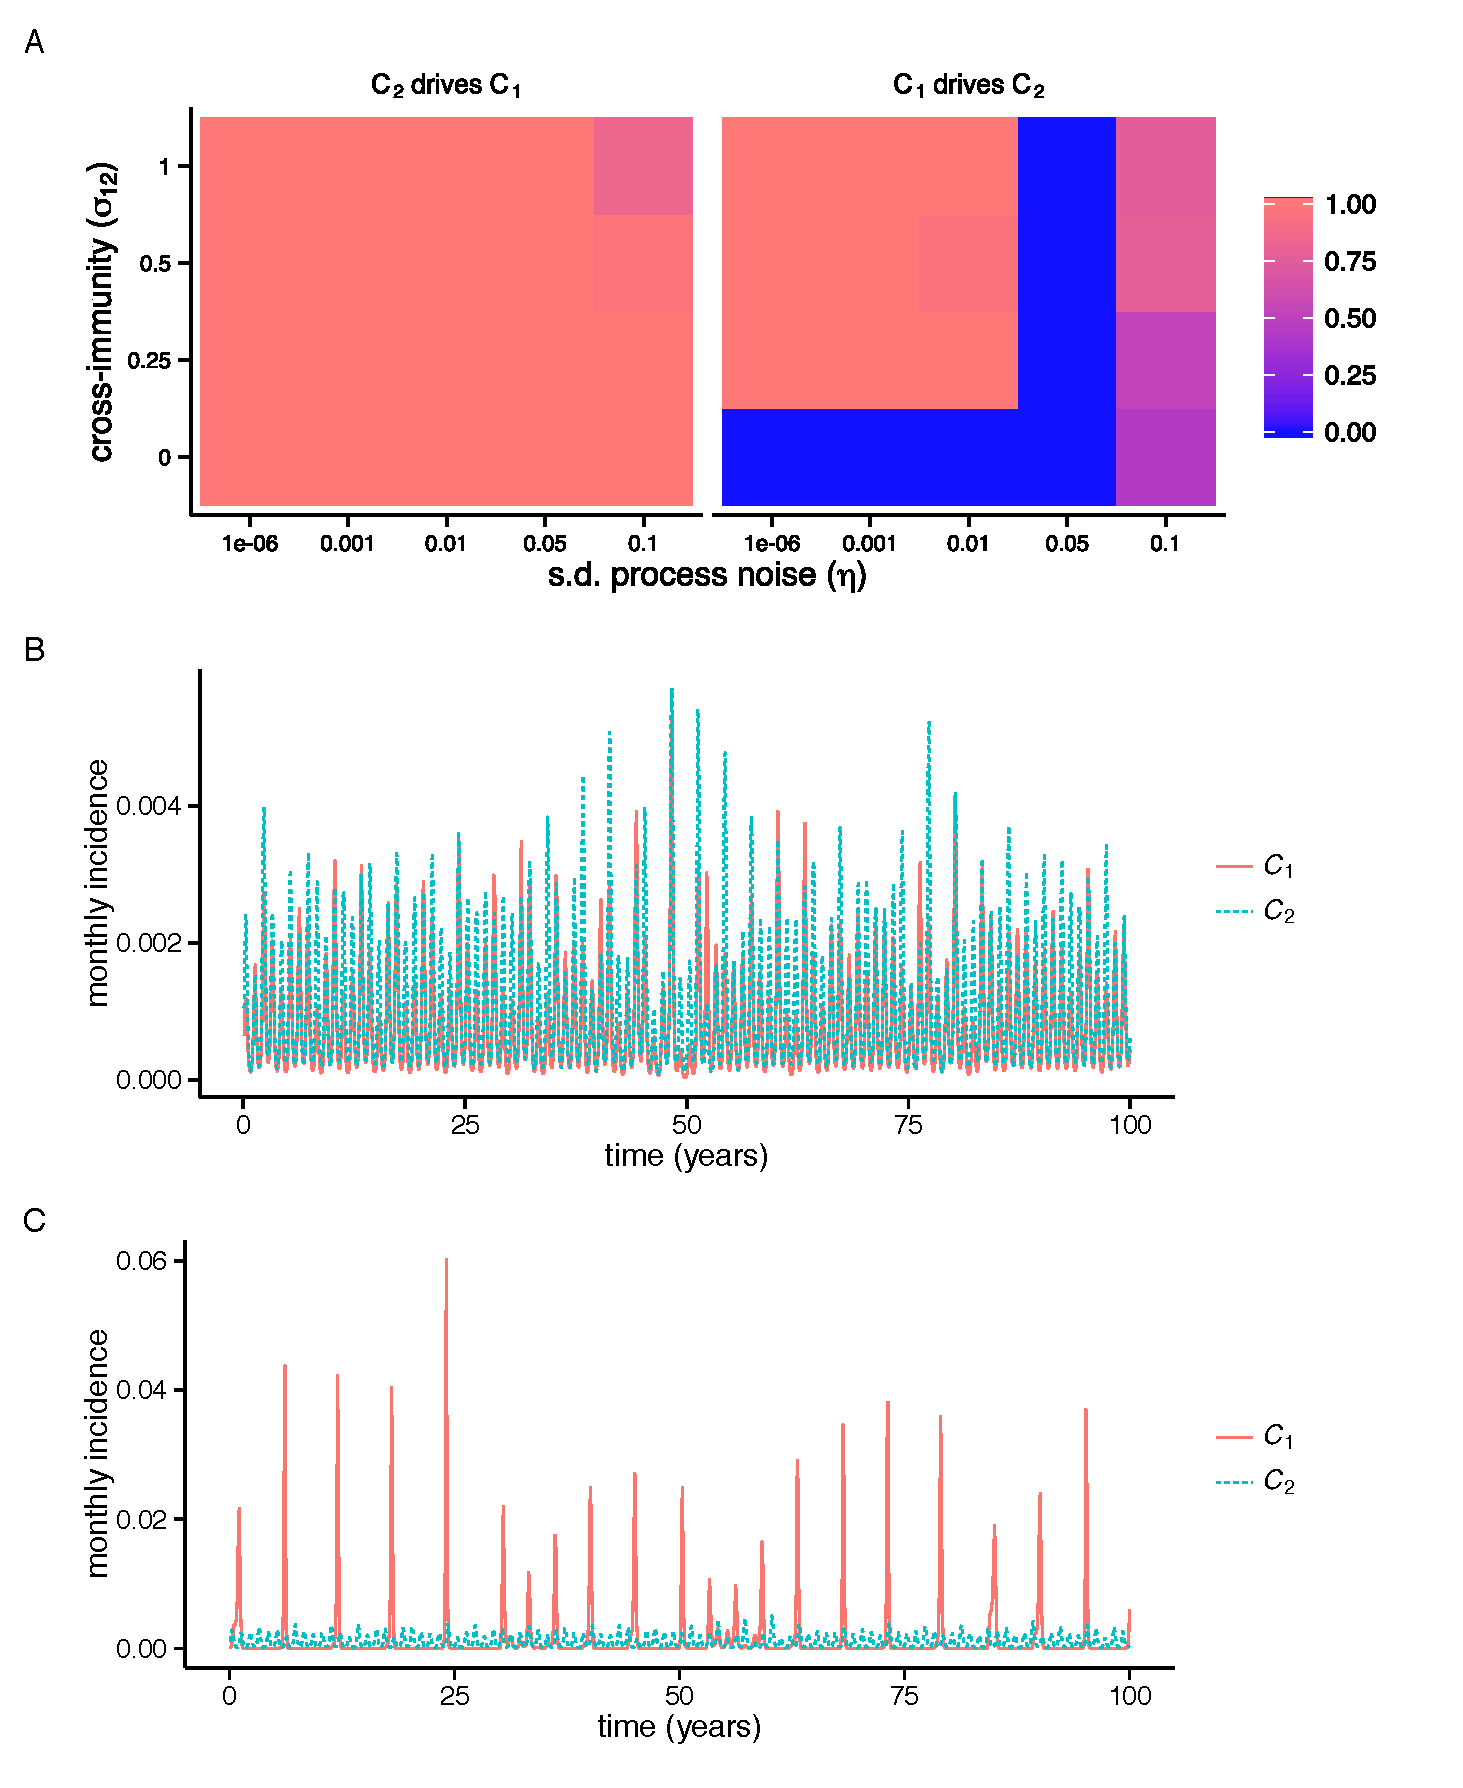
\includegraphics[width=5in]{dataflow/out/fig_detect_increase/fig_detect_increase.pdf}
  \end{center}
  \caption{\textbf{Interactions detected as a function of process noise and the strength of interaction ($C_2 \rightarrow C_1$) and representative time series}. (A) Heat maps show the fraction of 100 replicates significant for each inferred interaction for different parameter combinations. A significant increase in cross-map correlation $\rho$ with library length $L$ indicated a causal interaction. (B) Representative time series for which mutual interactions were inferred ($\sigma_{12}=0.25, \eta=0.01$). (C) Representative time series for which $C_2$ is inferred to drive $C_1$ but not vice-versa ($\sigma_{12}=0.25, \eta=0.05$).  \label{fig:univar_monthly_hm_tmp}} 
\end{figure}

The sensitivity of the method to periodicity persisted despite transformations of the data and changes to the  driver. 
One possible solution to reducing seasonal effects, sampling annual rather than monthly incidence, reduced the overall rate of false positives but also failed to detect some interactions (Fig. \ref{fig:crap_heatmaps_tmp}A).
Furthermore, when the effects of strain 2 on 1 were strongest, the reverse interaction was more often inferred.
Sampling the prevalence at annual intervals had similar results (Fig. \ref{fig:crap_heatmaps_tmp}B), and first-differencing the data did not qualitatively change outcomes (Fig. \ref{fig:crap_heatmaps_tmp}C).
The method yielded incorrect results even without seasonal forcing ($\epsilon=0$) because of noise-induced oscillations (Fig. \ref{fig:crap_heatmaps_tmp}D).
In all of these cases, the presence of shared periods between the strains correlated strongly and significantly with the rate of detecting a false interaction (Fig. \ref{fig:max_crossspec_tmp}).

Because cross-mapping skill should be sensitive to the quality of the reconstructed shadow manifolds, we investigated performance under other methods of constructing $\textbf{M}_{C_1}$ and $\textbf{M}_{C_2}$.
Nonuniform embedding methods allow the time delays to occur at irregular intervals, $\tau_1, \tau_2, ... \tau_{E-1}$, and this flexibility may provide a more parsimonious embedding of the dynamics.
Alternative methods of attractor reconstruction, including nonuniform embedding \cite{Nichkawde2013, Uzal2011}, random projection \cite{Tajima2015}, and maximizing the cross-map (rather than univariate) correlation failed to fix the problem (Fig. \ref{fig:crap_embeddings_tmp}).

\begin{figure}
\begin{center}
  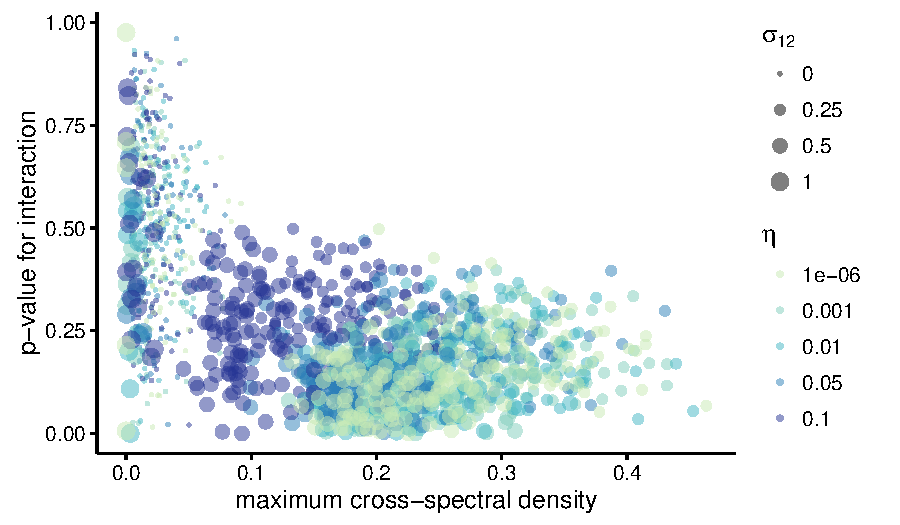
\includegraphics[width=5in]{dataflow/out/fig_spectra/fig_spectra.pdf}
  \end{center}
  \caption{\textbf{Shared frequency spectra predict probability of inferred interaction}. Points show the maximum cross-spectral densities of strains 1 and 2 plotted against the p-values for $C_1 \rightarrow C_2$. In all replicates, $C_1$ never actually drives $C_2$. Point color indicates the strength of $C_2 \rightarrow C_1$ ($\sigma_{12}$), and point size indicates the standard deviation of the process noise ($\eta$) on transmission rates. \label{fig:max_crossspec_tmp}} 
\end{figure}

The second criterion, which infers that $X$ drives $Y$ if there is a positive cross-map correlation $\rho$ (from $\textbf{M}_Y$ to $\textbf{M}_X$) that peaks at a negative cross-map lag, performed relatively well (Fig. \ref{fig:univar_monthly_lag_seas_diff_tmp}).
Fewer false positives were detected, although the method missed some weak extant interactions ($\sigma_{12}=0.25$) and interactions in noisy systems ($\eta=0.05, 0.1$).
Results for annual data were similar (Fig. \ref{fig:good_heatmaps_tmp}A).
Requiring that $\rho$ be not only positive but also increasing barely changed the performance (Fig. \ref{fig:good_heatmaps_tmp}B). 

\begin{figure}
\begin{center}
  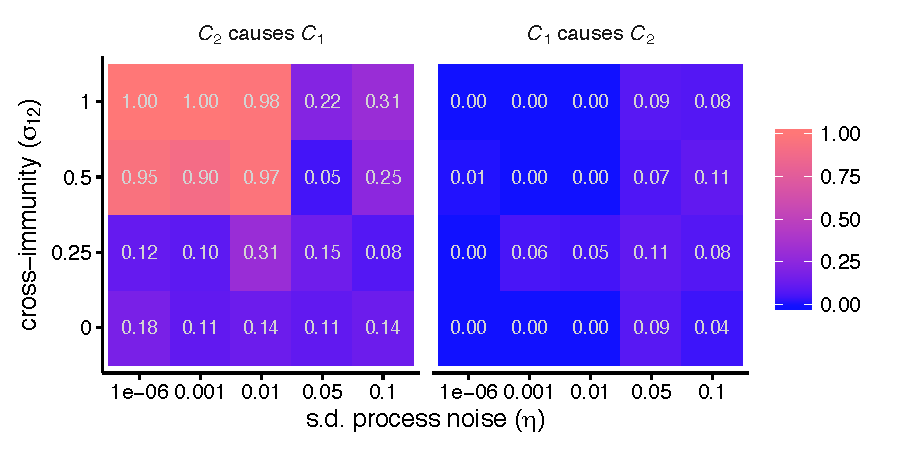
\includegraphics[width=5in]{dataflow/out/fig_detect_lag/fig_detect_lag.pdf}
  \end{center}
  \caption{\textbf{Interactions detected as a function of process noise and the strength of interaction ($C_2 \rightarrow C_1$) and representative time series}. Heat maps show the fraction of 100 replicates significant for each inferred interaction for different parameter combinations. A maximum, positive cross-map correlation $\rho$ at a negative lag indicated a causal interaction. Each replicate used 100 years of monthly incidence. \label{fig:univar_monthly_lag_seas_diff_tmp}} 
\end{figure}

\subsubsection{Limits to identifiability}

If two variables $X$ and $Y$ share the same driver but do not interact, at some limit, $X$ may resemble the driver so strongly that $X$ appears to drive $Y$.
In a similar vein, when the two strains in our system have identical reproductive rates ($\beta_1= \beta_2$) and one strongly drives the other ($\sigma_{12}=1$), the direction of the interaction cannot be detected when the dynamics are nearly deterministic ($\eta=10^{-6}$) (Fig. \ref{fig:good_heatmaps_tmp}C). 
Causal inference in such cases becomes difficult.

To investigate the limits to distinguishing ecologically similar, non-interacting strains, we varied the correlation of the strain-specific process noise while applying the more conservative criterion for inferring causality, that the cross-map correlation $\rho$ be positive and peak at a negative lag.
Process noise can be thought of as a hidden environmental driver that affects both strains simultaneously, and thus the strength of correlation indicates the relative contribution of shared versus strain-specific environmental noise.  
With two identical, independent strains and low process noise ($\eta=0.01$), the false positive rate varied non-monotonically with the correlation strength.
It peaked at approximately 19\%-24\% with perfectly correlated noise and reached a minimum at a correlation of 0.75 (Fig. \ref{fig:identical_corr_tmp}A).
Analyzing annual instead of monthly incidence, or applying the more stringent criterion that the maximum cross-map correlation $\rho$ not only be positive but also increase at a negative lag, reduced the false positive rate to $<5\%$ for imperfectly correlated noise (Fig. \ref{fig:identical_corr_tmp}B, C).
Thus, the independence of two strains will generally be detected as long as they experience imperfectly correlated noise. 

We next considered the problem of identifying two ecologically distinct strains ($\beta_1 \neq \beta_2$) when one strain strongly drives the other ($\sigma_{12}=1$) and its dynamics resemble the seasonal driver.
In this case, even with perfectly correlated process noise, correct interactions are consistently inferred (Fig. \ref{fig:diff_corr_tmp}).
Thus, we conclude that the presence of noise, even highly correlated noise, can help distinguish causality between coupled, synchronized variables.
It is more difficult to distinguish non-interacting, dynamically equivalent variables.
In the latter case, noise has inconsistent effects on causal inference, although more stringent criteria can help.
These results at least hold for ``modest" noise ($\eta=0.01$): as shown earlier, higher levels hurt performance (Fig. \ref{fig:univar_monthly_lag_seas_diff_tmp}).


\subsubsection{Non-steady-state dynamics}
CCM assumes steady-state dynamics, and deviations from steady-state should compromise the integrity of the shadow manifolds.
Our results have shown that the method is robust, and even benefits, from relatively low noise, but severe deviations from equilibrium behavior could limit effective cross-mapping.
As a proof of principle, we evaluated the impact of transient dynamics on causal inference.
When strain 2 weakly drives strain 1 ($\sigma_{12}=0.5$), the reverse interaction can be inferred instead (Fig. \ref{fig:nonstationary_tmp}).
In 100 simulations of this scenario at steady state, the correct interaction is inferred 100\% of the time, using the criteria that cross-map correlation $\rho$ be positive and maximized at negative lag.
With transient dynamics, the rate falls to approximately 80\%.
The true interaction ($C_2 \rightarrow C_1$) becomes more difficult to detect under the same circumstances (98\% with steady state and 80\% with transient dynamics).

\begin{figure}
\begin{center}
  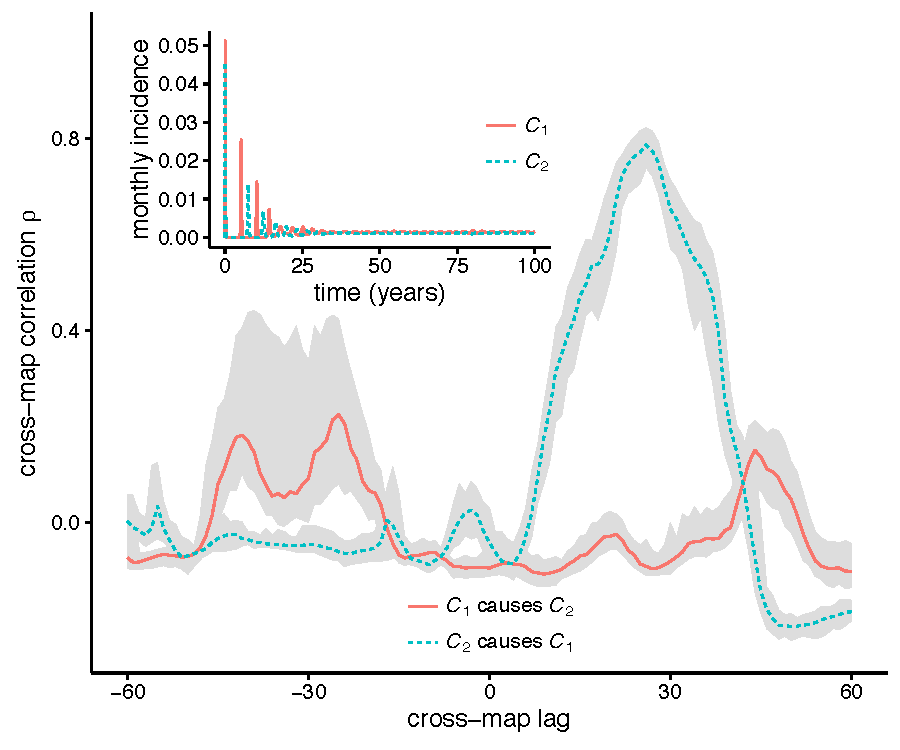
\includegraphics[width=5in]{dataflow/out/fig_transient/fig_transient.pdf}
  \end{center}
  \caption{\textbf{Incorrect inference with transient dynamics.} Cross-map correlations at different lags for a sample time series (inset). Although $C_2$ drives $C_1$ ($\sigma_{12}= 0.5, \sigma_{21}=0$), the maximum cross-correlation $\rho$ for $C_1$ cross-mapped to $C_2$ occurs at a positive lag, and the reverse at a negative lag, leading to the conclusion that $C_1$ drives $C_2$, and $C_2$ does not drive $C_1$. Sample dynamics include process noise ($\eta=0.01$) but no seasonal forcing ($\epsilon=0$). \label{fig:nonstationary_tmp}} 
\end{figure}

\subsubsection{Application to childhood infections}

Given the success of a modified form of CCM with two strains under some conditions, we investigated whether it might shed light on the historic dynamics of childhood infections in the pre-vaccine era.
We obtained the weekly incidence of six reportable infections in New York City from intermittent periods spanning 1906 to 1953 \cite{vanPanhuis2013} (Fig. \ref{fig:historical_data_tmp}A).
Six of 30 pairwise interactions were significant at the $p<0.05$ level, not correcting for multiple tests (Fig. \ref{fig:historical_data_tmp}C).
Polio drove mumps and varicella, scarlet fever drove mumps and polio, and varicella and pertussis drove measles. 
Typical cross-map lags occurred at one to three years (Fig. \ref{fig:nyc_uni_tmp}).
The inferred interactions were identical if we required that the cross-map correlation $\rho$ be increasing and not merely positive.

\begin{figure}
\begin{center}
  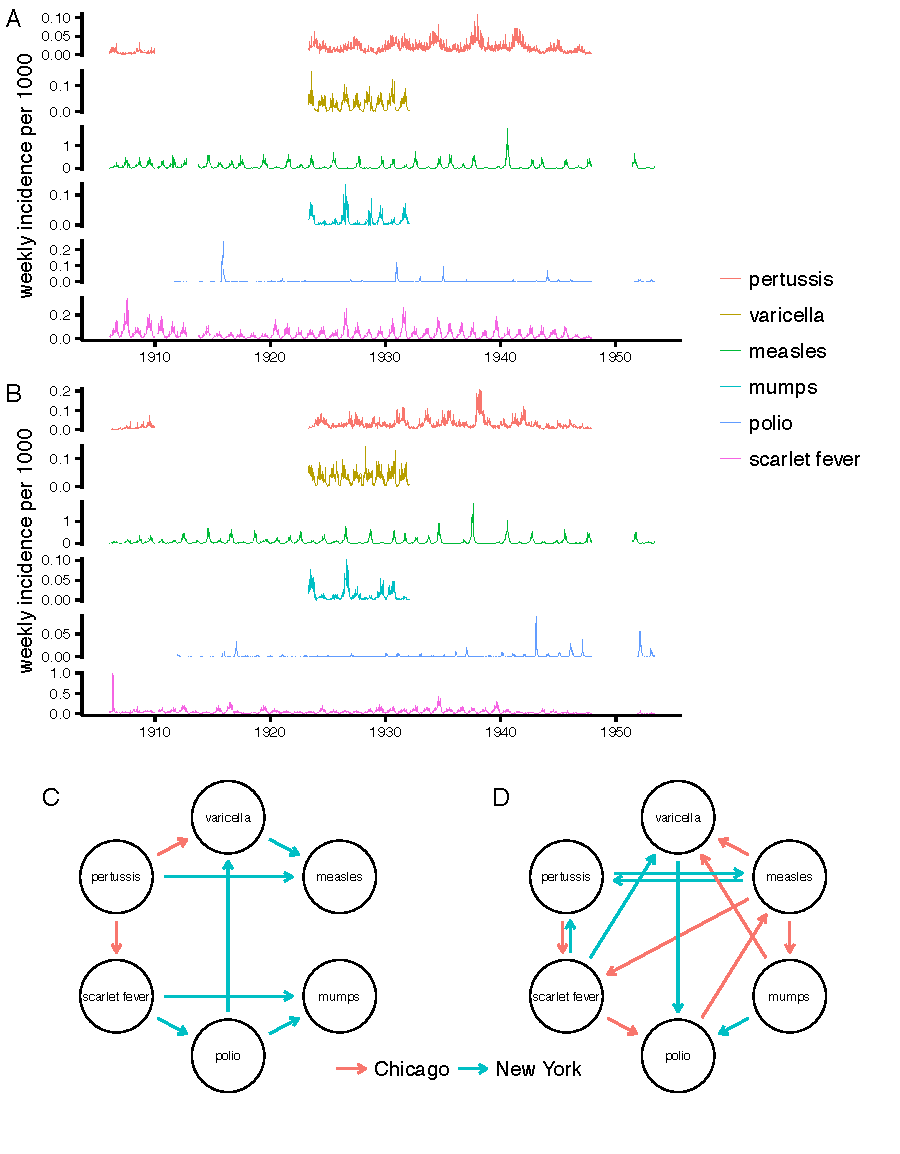
\includegraphics[height=5in]{dataflow/out/fig_cities/fig_cities.pdf}
  \end{center}
    \caption{\textbf{Historical childhood infections in New York City and Chicago and inferred interactions from two reconstruction methods.} Time series show weekly incidence of infections per 1000 inhabitants of New York City (A) and Chicago (B). Delay-embeddings were constructed by maximizing the univariate correlation (C) or through a random projection method (D) Arrows indicate the inferred interactions from the New York (blue) and Chicago (red) time series under the more stringent criterion (negative lag and increasing cross-map correlation).\label{fig:historical_data_tmp}} 
\end{figure}

Although we specifically chose infectious diseases not subject to major public health interventions in the sampling period, it is possible that the New York data reflect non-steady-state dynamics.
To the check robustness of the conclusions, we analyzed analogous time series from Chicago from the same period (Fig. \ref{fig:historical_data_tmp}B).
Completely different interactions appeared (Fig. \ref{fig:historical_data_tmp}C).
Not correcting for multiple tests, pertussis drove scarlet fever and varicella; accepting marginally significant negative lags ($p=0.055$), polio drove measles.
Requiring that the maximum cross-map correlation $\rho$ only be positive at negative lag, polio also drove pertussis, measles drove mumps and varicella, and mumps drove scarlet fever.
Except in one case, all negative lags occurred at more than one year (Fig. \ref{fig:chi_uni_tmp}).
Thus, no consistent interactions appeared from epidemiological time series of two major, and possibly dynamically coupled, cities.

To investigate the possibility that our method of attractor reconstruction might be unduly sensitive to noise and nonstationarity, we repeated the procedure with a method based on random projections \cite{Tajima2015}.
Once again, no interactions were common to both cities (Fig. \ref{fig:historical_data_tmp}D).
Only one of the original eight interactions from the original reconstruction method reappeared with random projection (two of eight reappeared if disregarding the city), and two interactions changed direction (three if disregarding the city). 
Similar lags were selected (Figs. \ref{fig:nyc_rand_tmp}, \ref{fig:chi_rand_tmp}).

\section{Discussion}

CCM is, in theory, an efficient alternative to mechanistic modeling for causal inference in nonlinear systems.
By evaluating properties of reconstructed attractors in state space, it sidesteps any need to formulate and fit what are usually inaccurate mathematical models.
In practice, CCM appears unsuitable for natural systems.
We simulated two interacting strains and found that traditional CCM can lead to erroneous conclusions whenever strains oscillated at similar frequencies.
Applying a different criterion for causality that considers the temporal lag at which cross-map correlation is maximized \cite{Ye2015}, rather than the change in cross-map correlation with time series length $L$ \cite{Sugihara2012}, avoids this problem.
Inference with this modified version of CCM is robust to relatively low process noise, which can actually improve performance.
But the method as a whole remains susceptible to deviations from its core assumptions. 
High process noise and non-steady-state dynamics each diminish performance, leading to false positives and negatives.
Because noise and nonequilibrium behavior are ubiquitous in nature, and there are currently no reliable methods to gauge their impact on the quality of state-space reconstruction, we propose CCM has no effective application for causal inference in natural systems.
These problems raise questions about the suitability of any method based on state-space reconstruction in ecology.

Oscillatory dynamics are common in nature, especially in infectious disease ecology, and suggest that the original criterion for causal inference might routinely mislead in ecological systems.
Climatic and seasonal cycles, driven by such factors as school terms, El Nino, and absolute humidity, pervade the dynamics of many pathogens and influence the timing of epidemics \cite{Shaman2010, Laneri2010, Finkenstadt2000, Altizer2006, Metcalf2009}. 
Infectious diseases exhibit periodic behavior in the absence of external forcing too.
These oscillations may arise from the well-known transient damped oscillations to equilibrium, but in nature, they perhaps arise more frequently from demographic stochasticity. 
This stochasticity induces fluctuations on characteristic time scales that can further interact with seasonal drivers to generate complex oscillatory patterns \cite{Alonso2006, Nguyen2008, Rand1991, Rohani2002}. 
Although we did not include demographic stochasticity in our model, with process noise acting on transmission, each strain developed a distinct frequency spectrum.
A tendency to cycle is not particular to infectious disease systems: other nonlinear systems incorporating consumer-resource interactions \cite{Boland2009, McKane2005, Turchin2003} or patchy populations \cite{Nisbet1978, Durrett1994} demonstrate similar behavior from stochastic effects alone.
However, there may be interesting differences in the tendency of discrete-time systems to undergo chaotic rather than periodic fluctuations, and these differences may affect the perceived performance of traditional CCM in different scenarios \cite{Sugihara2012}.

Assuming the stronger criterion for causality \cite{Ye2015}, under what conditions can we consider this method ``safe" for causal inference?
We have demonstrated that non-steady-state conditions pose one potential problem.
Although sometimes nonstationary or transient dynamics can be readily identified \cite{Ives2012}, and some forms of nonstationarity perhaps removed from the time series through first-differencing or detrending, not all forms of nonstationarity are identifiable or distinguishable from steady-state dynamics occurring over long time scales.
The lack of consistent bias (e.g., false negatives) from inference on nonstationary time series implies that this uncertainty might be a severe limitation for systems that are not already well understood.

If we were confident that the observed dynamics reflected steady-state behavior, the next challenge would be the selection of the delay-embedding for the shadow manifolds and the statistics for identifying the maximum cross-map correlations and negative lags.
Competing criteria for evaluating the quality of attractor reconstruction highlight the difficulty of justifying a particular delay-embedding \cite{Casdagli1991, Uzal2011, Nichkawde2013, Tajima2015, Sugihara1990}, which should become even more difficult in the presence of process noise.
Reconstructions from unknown systems thus run the risk of being ad hoc.
Because the delay-embedding influences the cross-map correlations $\rho$, causal inference could rest on slightly arbitrary decisions.   
This arbitrariness currently extends to our identification of significant increases in cross-map correlations, or significantly negative cross-map lags.
We bootstrapped and attempted to validate the approach empirically with simulated data, but this heuristic differs starkly from the likelihood-based approaches common to mechanistic modeling \cite{HilbornMangel}.

Noise and non-steady-state dynamics could explain the contrasting results for childhood infections in two cities. 
Although there is evidence that measles increases suceptibility to other infections \cite{Mina2015}, and that measles and pertussis compete for susceptible hosts \cite{Rohani2003}, the time series did not strongly support these hypotheses. 
Furthermore, it is difficult to imagine a parsimonious mechanism by which the inferred interactions might be biologically consistent and plausible.
Different rates or modes of transmission for each disease in each city might lead to varying patterns of infection in different subpopulations, affecting interactions.
However, we know of no support for this hypothesis.
In contrast, we could not rule out nonstationarity in the dynamics, which we might expect from changes in birth rates, mobility, and behavior during this period \cite{Earn2000}.
High process noise, implying the omission of important state variables and poor resolution of the underlying attractor, hurt the performance of CCM and could also affect inference in this case. 
Errors in attractor reconstruction are another possibility. 
Except for pertussis, different delay-embeddings were selected for each pathogen in each city, and an alternative method of attractor reconstruction yielded even more divergent results. 


While the statistical foundations of attractor reconstruction are in development, perhaps the most appropriate use of CCM is for exploratory analysis.
In steady-state systems, causal inference appears reliable when based on the temporal lag at which the cross-map correlation peaks \cite{Ye2015}.
Because many populations, especially of hosts and pathogens, are evolving and undergoing strong directional changes, inference from state-space reconstruction must be extended carefully.
Mechanistic models remain the only option for predicting out-of-sample dynamics in rapidly evolving systems, and they may  prove more reliable for causal inference in these cases too.
The balance hangs partly on the degree to which natural processes are fundamentally ordered and at equilibrium \cite{Hastings2004}.

\section{Acknowledgements}
We thank Mercedes Pascual, Greg Dwyer, and Nicolas Brunel for helpful comments.

\section{Materials and Methods}

\subsection{Dynamical model}
We modeled the dynamics of two pathogen strains under variable amounts of competition and process noise.
The state variables in the system are the hosts' statuses with respect to each strain \cite{Gog2002}. 
Hosts can be susceptible ($S_i$), infected ($I_i$), or recovered and immune ($R_i$) to each strain $i$. 
The deterministic model has the form:

\begin{align}
\frac{dS_i}{dt} &=
    \mu
    - S_i\sum\limits_{j}
    \sigma_{ij}
    \beta_j(t) 
    I_j
    - \mu S_i \\
\frac{dI_i}{dt} &= 
    \beta_i(t) S_i I_i
    - (\nu_i + \mu) I_i \\
\frac{dR_i}{dt} &=
    \nu_i I_i
    + S_i\sum\limits_{j \neq i} \sigma_{ij} \beta_j(t)  I_j
    - \mu R_i \\
\beta_i(t) &= \beta_i
    \left(
        1 + \varepsilon \sin \left[
            \frac{2\pi}{\psi} \left( t - \psi \right)
        \right]
    \right) \\
S_i + I_i + R_i &= 1
\end{align}

Hosts enter the susceptible class for strain $i$ through the birth (and death) rate $\mu$. 
They leave through infection with strain $i$ ($S_i \to I_i$), infection with strain $j$ that elicits cross-immunity to $i$ ($S_i \to R_i$), or death.
The per capita transmission rate, $\beta_i(t)$, depends on a mean strain-specific rate, $\beta_i$, and a sinusoidal forcing function defined by a shared period, $\psi$. 
The amplitude of forcing, $\epsilon$, is constant across strains. 
Infected hosts recover at rate $\nu_i$ ($I_i \to R_i$).
The immune host class grows through these recoveries and also from the fraction of susceptible hosts, $S_i$, contacting infected hosts, $I_j$, who develop cross-immunity, $\sigma_{ij}$ ($0<\sigma_{ij}<1$).
Immunity of this form has been described as ``polarizing" because $\sigma_{ij}$ of hosts $S_i$ contacting infecteds $I_j$ become completely immune (non-susceptible) to strain $i$, while $1-\sigma_{ij}$ remain completely susceptible.
This cross-immunity is a form of competition that determines the directions of interaction between strains: when $\sigma_{ij}>0$, strain $j$ drives strain $i$.

Process noise on the per capita transmission rate produces stochastic differential equations in Ito form:
\begin{align}
dS_i &=
	[\mu - \mu S_i] \, dt
	- S_i\sum\limits_{j} \sigma_{ij} \beta_j(t) I_j [dt +\eta \, dW_{t,j}] 
	\\
dI_i &= 
	\beta_i(t) S_i I_i [dt +  \eta \, dW_{t,i}]
	- [\nu_i + \mu] I_i \,  dt \\
dR_i &=
	[\nu_i I_i - \mu R_i] \, dt
	+ S_i\sum\limits_{j \neq i} \sigma_{ij} \beta_j(t) I_j [dt +  \eta \, dW_{t,j}]
\end{align}
where the $W_i$ are independent Wiener processes, one for each pathogen $i$, and $\eta$ represents the standard deviation of the noise as a fraction of the deterministic transmission rate.

The observations consist of the number of new cases or incidence over some interval. 
Cumulative cases $c_i$ at time $t$ were obtained by summing the $S_i \to I_i$ transitions from the start of the simulation through time $t$.
The incidence over times $t-\Delta t_\text{obs}$ to $t$, written as $C(t)$ for convenience, is given by the difference in cumulative cases:
\begin{align}
C_i(t) &= c_i(t_2) - c_i(t_1) \\
dc_i &= \beta_i(t) S_i I_i [dt + \eta \, dW_{t,i}]
\end{align}


\subsection{Simulation}

The equations were solved numerically using the Euler-Maruyama method with a fixed step size. 
The step size was chosen to be less than the smallest within-run harmonic mean step size across deterministic, adaptive-step size pilot runs performed across the range of parameter space being studied. 
When numerical errors arose during transients, the step size was reduced further until the numerical issues disappeared.

Except where noted, the model was simulated with random initial conditions, and 1000 years of monthly observations were obtained from steady state conditions.
The use of random initial conditions minimizes arbitrary bias in the simulated dynamics.
From visual inspection of dynamics, the transient phase lasted much less than 1000 years. Time series were obtained from years 2000-3000.


\subsection{Cross-mapping}

In its most general form, CCM evaluates predictions of states of $X$ given observations of $Y$. 
When the system is stationary, two bidirectionally coupled variables $X$ and $Y$ share an attractor and contain complete information about the attractor in their time series.
We denote this attractor $\pmb{M}$ and the shadow manifolds of individual state variables $\pmb{M}_X$, $\pmb{M}_Y$, and so on.
To evaluate whether $X$ drives $Y$, we first construct shadow manifolds $\pmb{M}_Y$ from the time series of $Y$. 
Each point in $\pmb{M}_Y$ is given by an $E$-dimensional vector $\vec{y}(t)$ = \{$Y_t, Y_{t-\tau}, Y_{t-2\tau},...,Y_{t-(E-1)\tau}$\}, where $E$ is the embedding dimension and $\tau$ is the delay.
A total of $L$ points, referred to as the ``library``, are used to construct $\pmb{M}_Y$, and these points are the basis for predictions of states of $X$.
Each point in the time series of $X$ has an analogue on its own manifold $\pmb{M}_X$, i.e., an $E$-dimensional vector $\vec{x}(t)$ = \{$X_t,...,X_{t-(E-1)\tau}$\}. 
For each point in the time series of $X$, $X(t)$, we identify the contemporaneous point $\vec{x}_t$ in $\pmb{M}_X$ and $\vec{y}_t$ in $\pmb{M}_Y$.
For $\vec{y}_t$, we identify the point's $E$+1 nearest neighbors.
These neighbors (but not $\vec{y}_t$ itself) are then used to derive weights for a prediction of $X$, $\hat{X}(t)$. 
Specifically, the $E$+1 nearest neighbors of $\vec{y}_t$ are each weighted by their Euclidean distances to $\vec{y}_t$ \cite{Sugihara2012}, so that the unnormalized weight for neighbor $i$ at distance $d_i$ is $\exp\left(-\frac{d_i}{d_0} \right)$, where $d_0$ is the distance to the nearest neighbor.
In order to avoid predictability due to system autocorrelation rather than dynamical coupling, nearest neighbors were restricted to be greater than $dt_{\mathrm{neighbor}} = 3dt_{\mathrm{autocorr}}$ samples apart in time, where $dt_{\mathrm{autocorr}}$ is the delay at which the time-series autocorrelation drops below $1/e$.
To predict $\hat{X}_t$, these weights are then multiplied by the respective points in $\pmb{M}_X$ that are contemporaneous to each of the nearest neighbors of $\vec{y}_t$.
The cross-map correlation $\rho$ is computed by comparing the predicted ($\hat{X}(t)$) and actual ($\vec{x}_t$) values over the entire time series of $X$.

Libraries consisting of different points will produce different predictions, and thus define a distribution over $\rho$. We sample the $L$ delay vectors of $Y$ in the library randomly with replacement to yield a single library. We perform this sampling, and the corresponding cross-map prediction, many times to construct a bootstrap distribution for $\rho$ as the basis of statistical tests.

\subsection{Criteria for causality}

We infer causality using three different criteria involving $\rho$ \cite{Sugihara2012, Ye2015}: (1) whether $\rho$ increases with $L$; (2) whether $\rho$ is positive at $L = L_{\max}$, and (3) when cross-mapping the driven variable to different lags (temporal offsets) of the driver, whether $\rho$ is maximized at a negative lag.

If $X$ drives $Y$, $\pmb{M}_Y$ cross-maps to $\pmb{M}_X$, and increasing the density of the shadow manifold $\pmb{M}_Y$ by increasing $L$ should improve predictions of $\vec{x}_t$ and increase $\rho$ \cite{Sugihara2012}.
The first criterion tests for this increase in $\rho$ with $L$.
An increase in $\rho$ is indicated by a lack of overlap between the distributions at $L_{\min} = E + 2$, the smallest library that will have $E + 1$ neighbors for most points, and $L_{\max}$, the largest possible library given the time-series length and delay embedding parameters $E$ and $\tau$.


The second criterion relaxes the requirement of an increase in $\rho$, and instead simply requires that $\rho$ be positive at $L_{\max}$.

The third criterion requires that for $X$ to drive $Y$, $\rho$ (from $\pmb{M}_Y$ cross-mapped to $\pmb{M}_X$) is both positive and peaks at a negative cross-map lag \cite{Ye2015}.
In other words, not only must $M_Y$ contain information about $M_X$ ($\rho > 0$), but this information must be greatest for past states of $X$, reflecting the correct temporal direction for causality.
Replicates were also used to evaluate $\rho$ at each possible cross-map lag. 


\subsection{Statistical tests for causality criteria}

The theory underlying CCM assumes completely deterministic interactions and infinite data.
If $X$ drives $Y$ in the absence of noise, the correlation $\rho$ between the predicted and observed states of $X$ should converge to one with infinite samples of $Y$.
In practice, if $X$ and $Y$ share a complex (e.g., chaotic) attractor, time series of $Y$ may not be long enough to see convergence \cite{Sugihara2012}.

The presence of observation and/or process noise violates the deterministic assumptions and prevents $\rho$ from ever reaching one.
Nonetheless, a detectable increase in the correlation $\rho$ with the library length $L$ used to construct $\pmb{M}_Y$ (for the first criterion), a detectable positive value of $\rho$ (for the second criterion), or a maximum correlation at negative lag (for the third criterion), may suffice to demonstrate that $X$ drives $Y$ in natural systems.
It is important to note that we have no formal theoretical justification for such statistical heuristics.

Our statistics are based on the distributions obtained from bootstrapping.
For the first criterion, which tests for an increase in $\rho(L)$, we perform a nonparametric test of whether $\rho(L_{\max})$, obtained at the largest library length is greater than $\rho(L_{\min})$, obtained at the smallest libary length.
The p-value for this test is calculated as the probability that $\rho(L_{\max})$ is not greater than $\rho(L_{\min})$, and calculate the p-value directly from the sampled distributions.

For the second criterion, we simply test whether $\rho$ is detectably positive. The p-value for this test is simply the probability, based on the bootstrap distribution of $\rho$, that $\rho$ is positive.

For the third criterion, which tests whether the best cross-map lag is negative and thus indicates the correct causal direction in time, we perform a similar nonparametric test.
We identify the negative cross-map lag $\ell^{(-)}$ with the highest median correlation, $\rho(\ell^{(-)})$ as well as the nonnegative cross-map lag $\ell^{(0+)}$ with the highest median correlation.
The p-value for this test is calculated as the probability that $\rho(\ell^{(-)})$ is not greater than $\rho(\ell^{(0+)})$.

\subsection{Choice of delay and embedding dimension}
Attractor reconstruction is an unsolved problem \cite{Casdagli1991}.
The manifold $\pmb{M}$ is defined in $E$-dimensional state space, and the shadow manifolds are similarly defined by $E$ and some delay $\tau$.
In simulated, deterministic models, $E$ can be known perfectly.
In systems with process noise, unknown dynamics, and/or finite observations, there is no clearly superior method to select the appropriate embedding dimension and delay \cite{Casdagli1991,Nichkawde2013,Uzal2011,Pecora2007, Cao1997, Small2004}.

We accommodated this uncertainty by using four different methods.
Two methods infer the best delay-embedding for each interaction by maximizing the ability of one variable, the driven variable, to predict itself (akin to nonlinear forecasting \cite{Sugihara1990, Sugihara1994}).
The third method instead uses the delay-embedding that maximizes the cross-mapping correlation $\rho$ for each interaction.
Three of the four methods use uniform embeddings, identifying $E$ and a fixed delay $\tau$, and the other uses a nonuniform embedding, identifying a series of specific delays $\tau_1$, $\tau_2$, etc., whose length determines $E$.

\begin{enumerate}
\item \textit{Univariate prediction method}: By default, for each causal interaction ($C_i \rightarrow C_j$), $E$ and $\tau$ are chosen to maximize the one-step-ahead univariate prediction $\rho$ at $L_{\max}$ for the driven variable ($C_j$) based on its own time series.
\item \textit{Maximum cross-correlation method}: As an alternative, $E$ and $\tau$ are chosen to maximize the mean cross-map correlation $\rho$ at $L_\text{max}$ for each causal interaction being tested, for each time series.
\item \textit{Random projection method}: A recently proposed method based on random projection of delay coordinates sidesteps the problem of choosing optimal delays \cite{Tajima2015}. Instead, for a given $E$, all delays up to a maximum delay $\tau_{\max}$ are projected onto an $E$-dimensional vector via multiplication by a random projection matrix. $E$ is chosen to maximize the cross-map correlation $\rho$.
\item \textit{Nonuniform method}: For each driven variable $C_j$, starting with $\tau_0 = 0$, additional delays $\tau_1, \tau_2, \ldots$ are chosen iteratively to maximize the directional derivative to nearest neighbors when the new delay is added \cite{Nichkawde2013}. The delays are bounded by the optimal uniform embedding based on a cost function that penalizes irrelevant information \cite{Uzal2011}. This method can be seen as a nonuniform extension of the method of false nearest neighbors \cite{Kennel1992}.
\end{enumerate}


\subsection{Code}
Code implementing the state-space reconstruction methods is publicly available at \url{https://github.com/cobeylab/pyembedding}.
The complete code for the analysis and figures is publicly available at \url{https://github.com/cobeylab/causality_manuscript}; individual analyses include references to the Git commit version identifier in the `pyembedding` repository.
The simulated time series on which the analyses were performed are available from the authors on request.

\subsection{Data on childhood infections}
Time series were obtained from L2-level data maintained by Project Tycho \cite{vanPanhuis2013}.
All available cases of measles, mumps, pertussis, polio, scarlet fever, and varicella were obtained from the first week of 1906 through the last week of 1953 for New York City and Chicago.
Pertussis data were truncated at the start of 1948.
Incidence was calculated by dividing weekly cases by a spline fit to each city's population size, as reported by the U.S. Census.

\bibliography{ccm_ms}

\begin{table}
\caption{Default parameter values.}
\begin{center}
\begin{tabular}{cccc}
{\bf Symbol} &{\bf Description} & {\bf Default value} \\ 
\hline
$\beta_1, \beta_2$ & transmission rates & 0.3, 0.25 $\text{d}^{-1}$ \\
$\sigma_{12}$ & immunity to strain 1 from infection with 2 & see text\\
$\sigma_{21}$ & immunity to strain 2 from infection with 1 & 0\\
$\sigma_{ii}$ & homologous immunity for strain $i$ & 1\\
$\mu$ & birth and death rate & 1/30 $\text{y}^{-1}$ \\
$\nu$ & recovery rate & 0.2 $\text{d}^{-1}$ \\
$\epsilon$ & amplitude of seasonal forcing & 0.1 \\
$\psi$ & period of seasonal forcing & 360 d\\
$\eta$ & standard deviation of process noise & see text \\
$\text{S(0)}$ & initial fraction susceptible & see text \\
$\text{I(0)}$ & initial fraction infected & see text\\
$\Delta t_\text{obs}$ & incidence and sampling interval & 30 days\\
\end {tabular}
\end{center}

\label{table:defaultParameters}
\end {table}

\beginsupplement
\section{Supplement}

\begin{figure}
\begin{center}
  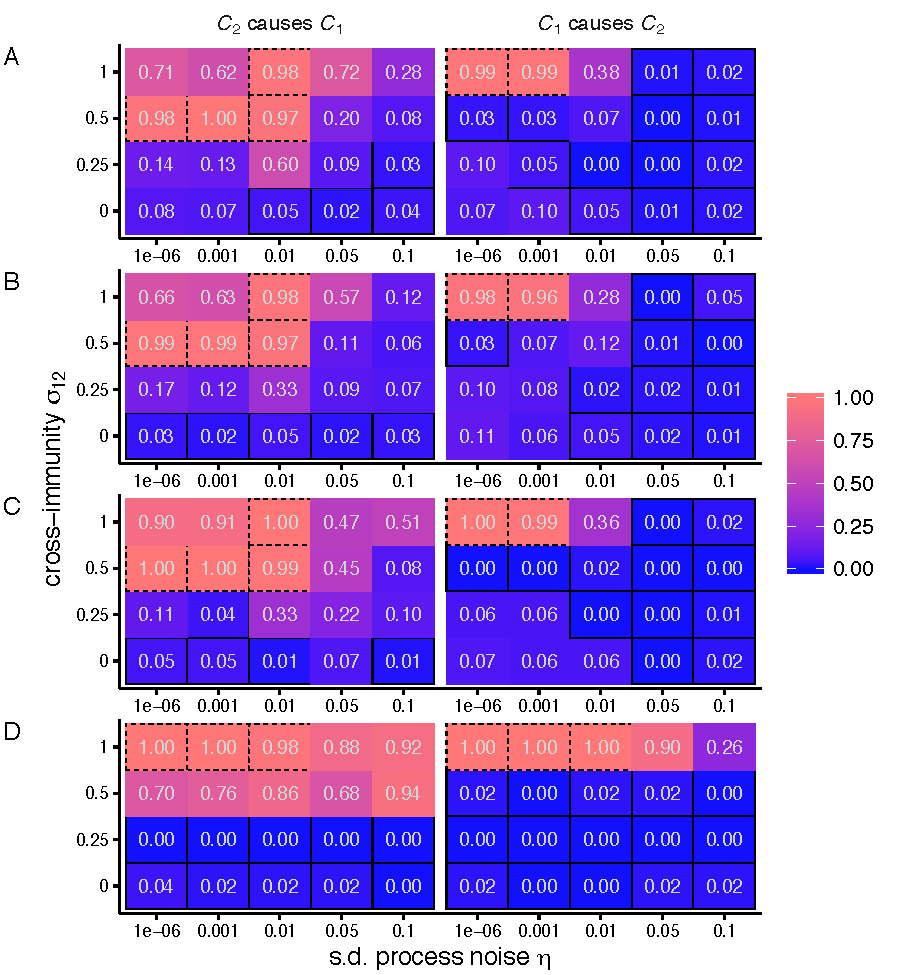
\includegraphics[width=3.5in]{dataflow/out/fig_detect_diffdata/fig_detect_diffdata.pdf}
  \end{center}
  \caption{\textbf{Interactions detected as a function of process noise and the strength of interaction ($C_2 \rightarrow C_1$) for different types of data}. Heat maps show the fraction of 100 replicates significant for each inferred interaction for different parameter combinations. A significant increase in cross-map correlation $\rho$ with library length $L$ indicated a causal interaction. (A) Annual incidence, (B) prevalence strobed annually, (C) first-differenced annual incidence, and (D) monthly incidence without seasonal forcing.  \label{fig:crap_heatmaps_tmp}}
\end{figure}


\begin{figure}
\begin{center}
  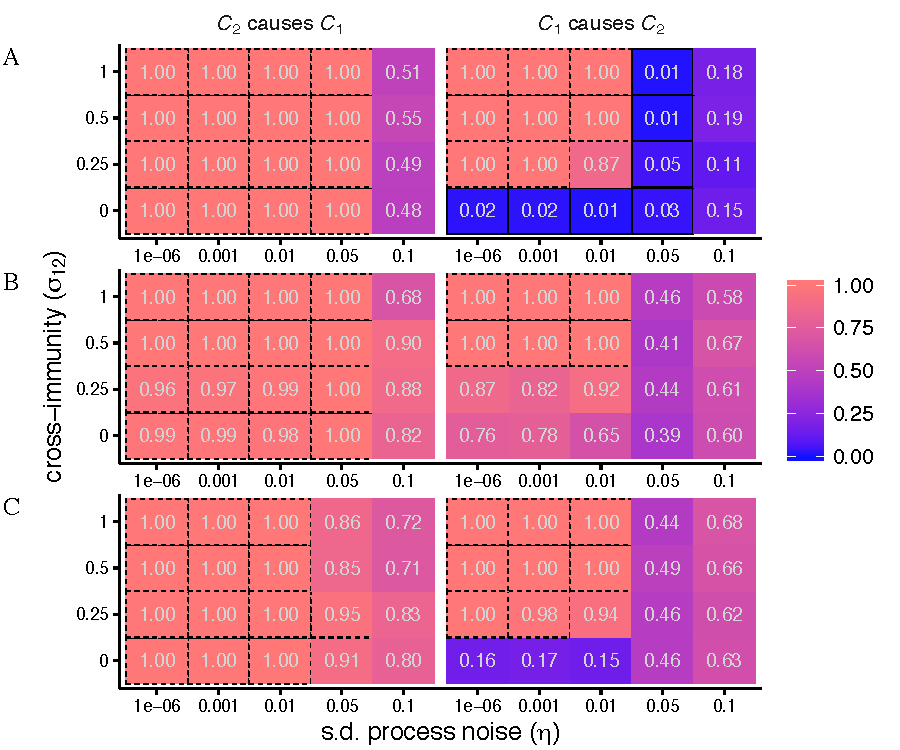
\includegraphics[width=5in]{dataflow/out/fig_detect_diffembed/fig_detect_diffembed.pdf}
  \end{center}
  \caption{\textbf{Interactions detected as a function of process noise and the strength of interaction ($C_2 \rightarrow C_1$) for different delay-embedding methods}. Heat maps show the fraction of 100 replicates significant for each inferred interaction for different parameter combinations. A significant increase in cross-map correlation $\rho$ with library length $L$ indicated a causal interaction. Delay-embeddings were chosen by (A) nonuniform embedding, (B) random projection, or (C) maximizing the cross-map correlation $\rho$.  \label{fig:crap_embeddings_tmp}}
\end{figure}

\begin{figure}
\begin{center}
  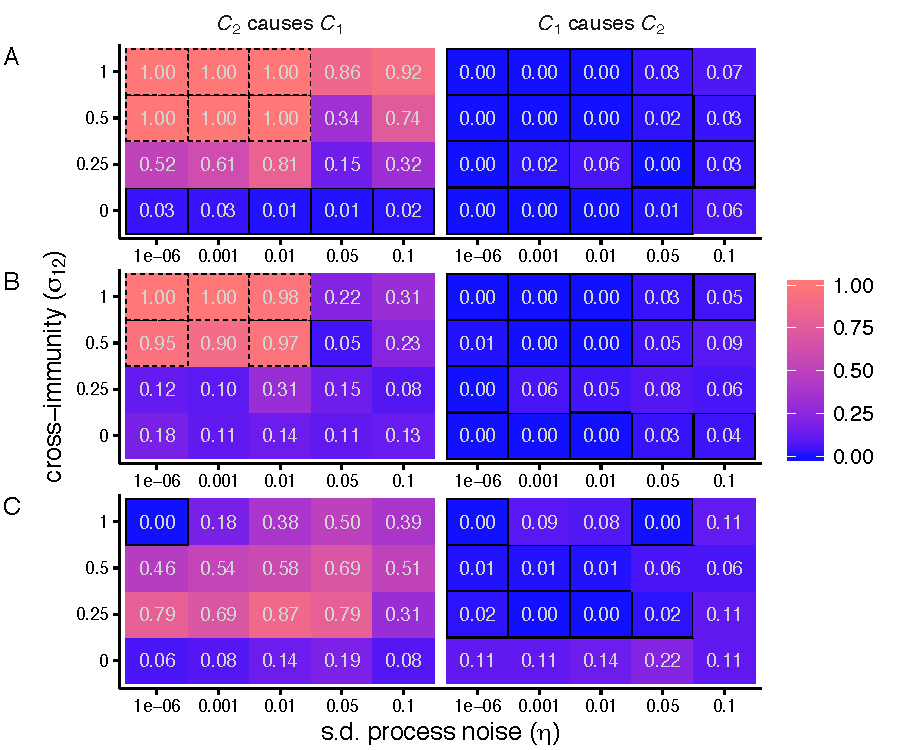
\includegraphics[width=5in]{dataflow/out/fig_detect_diffdata_lag/fig_detect_diffdata_lag.pdf}
  \end{center}
  \caption{\textbf{Interactions detected for different types of data}. Heat maps show the fraction of 100 replicates significant for each inferred interaction for different parameter combinations. A maximum cross-map correlation $\rho$ at a negative lag was required for inferring causal interaction. (A) Annual incidence, requiring that the maximum $\rho$ be positive. (B) Monthly incidence, requiring that the maximum $\rho$ be increasing. (C) Monthly incidence with identical strains ($\beta_1=\beta_2=0.3$), requiring that maximum $\rho$ be positive.  \label{fig:good_heatmaps_tmp}}
\end{figure}

\begin{figure}
\begin{center}
  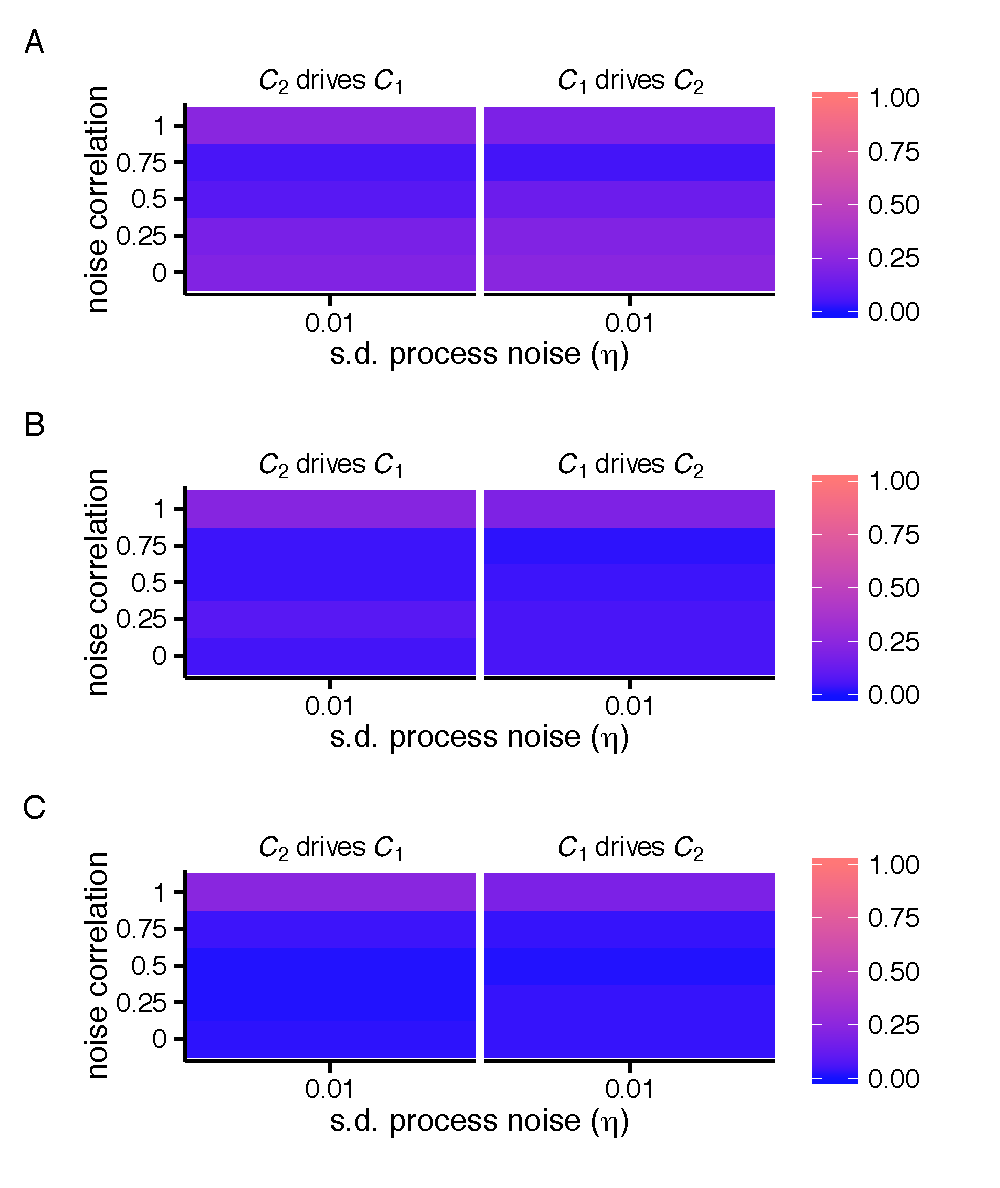
\includegraphics[width=5in]{dataflow/out/fig_detect_corrproc_identical/fig_detect_corrproc_identical.pdf}
  \end{center}
  \caption{\textbf{Interactions detected between identical strains with correlated process noise}. Heat maps show the fraction of 100 replicates significant for each inferred interaction. A maximum cross-map correlation $\rho$ at a negative lag was required for inferring causal interaction. Monthly (A) and annual (B) incidence, requiring that the maximum $\rho$ be positive. (C) Monthly incidence, requiring that maximum $\rho$ be increasing.  \label{fig:identical_corr_tmp}}
\end{figure}

\begin{figure}
\begin{center}
  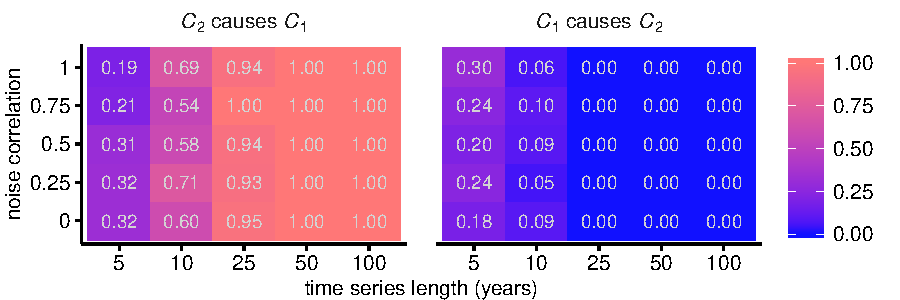
\includegraphics[width=5in]{dataflow/out/fig_detect_corrproc_distinct/fig_detect_corrproc_distinct.pdf}
  \end{center}
  \caption{\textbf{Interactions detected between distinct strains with correlated process noise}. Heat maps show the fraction of 100 replicates significant for each inferred interaction. A maximum cross-map correlation $\rho$ at a negative lag and $\rho>0$ were required for inferring causal interaction. Results shown for monthly incidence.  \label{fig:diff_corr_tmp}}
\end{figure}

\begin{figure}
\begin{center}
  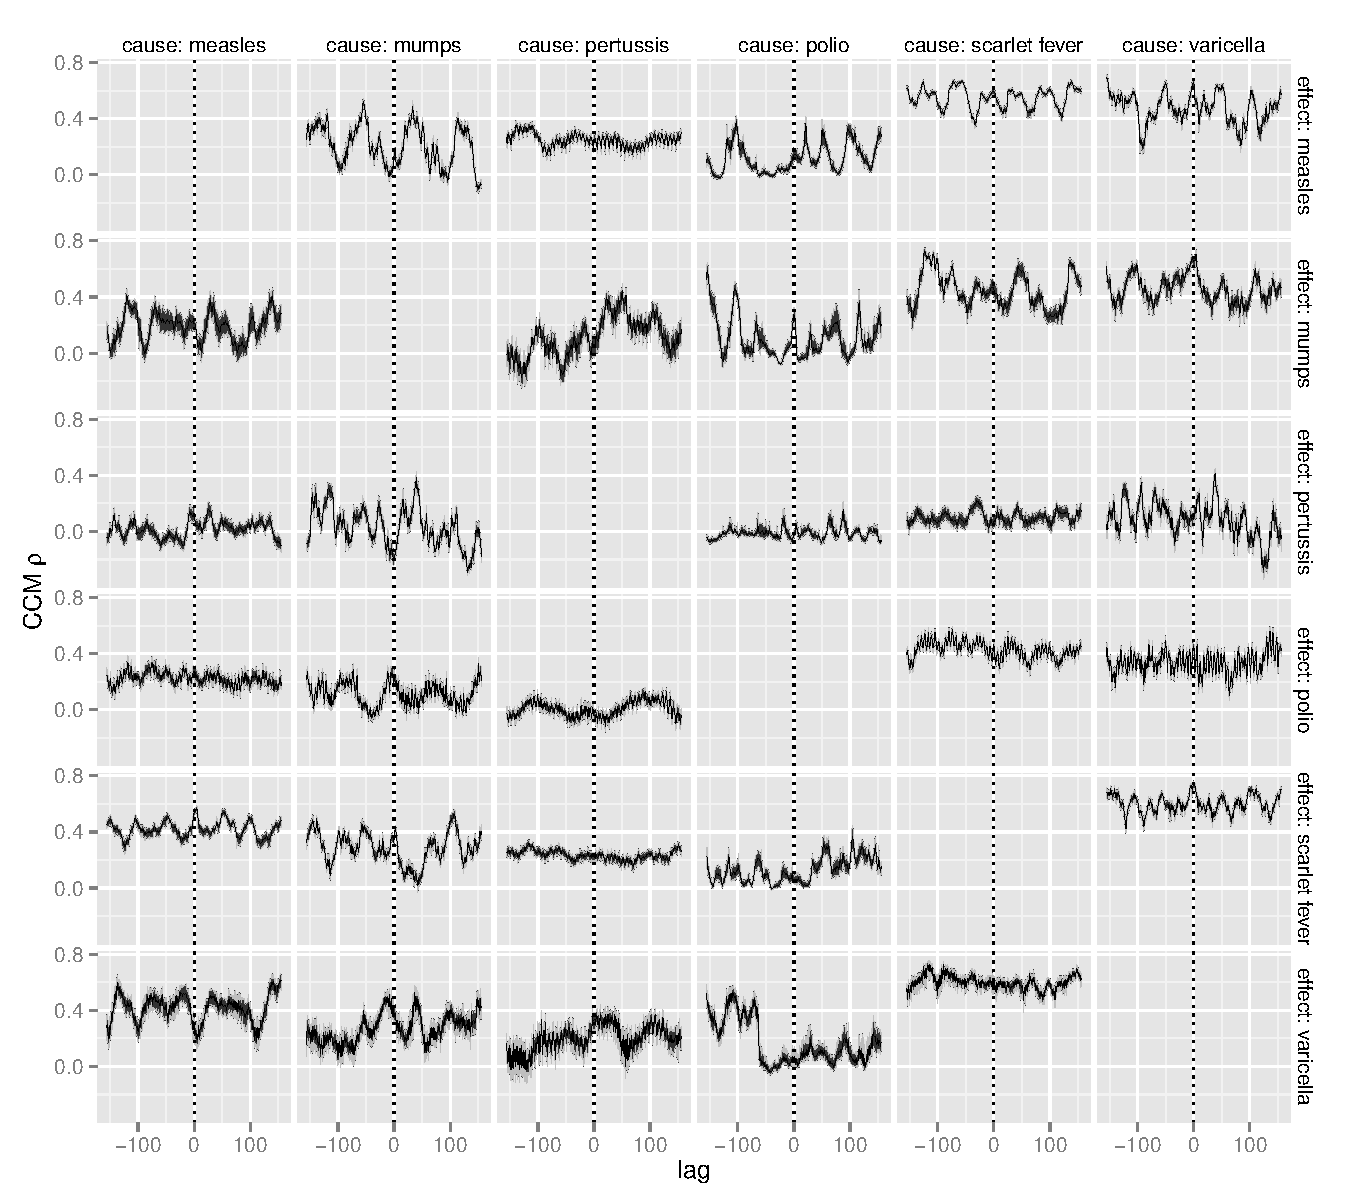
\includegraphics[width=5in]{dataflow/out/fig_cities_corrbylag/nyc_self_uniform_plot.pdf}
  \end{center}
  \caption{\textbf{Cross-map lags for New York with default (univariate) embedding}.  \label{fig:nyc_uni_tmp}}
\end{figure}

\begin{figure}
\begin{center}
  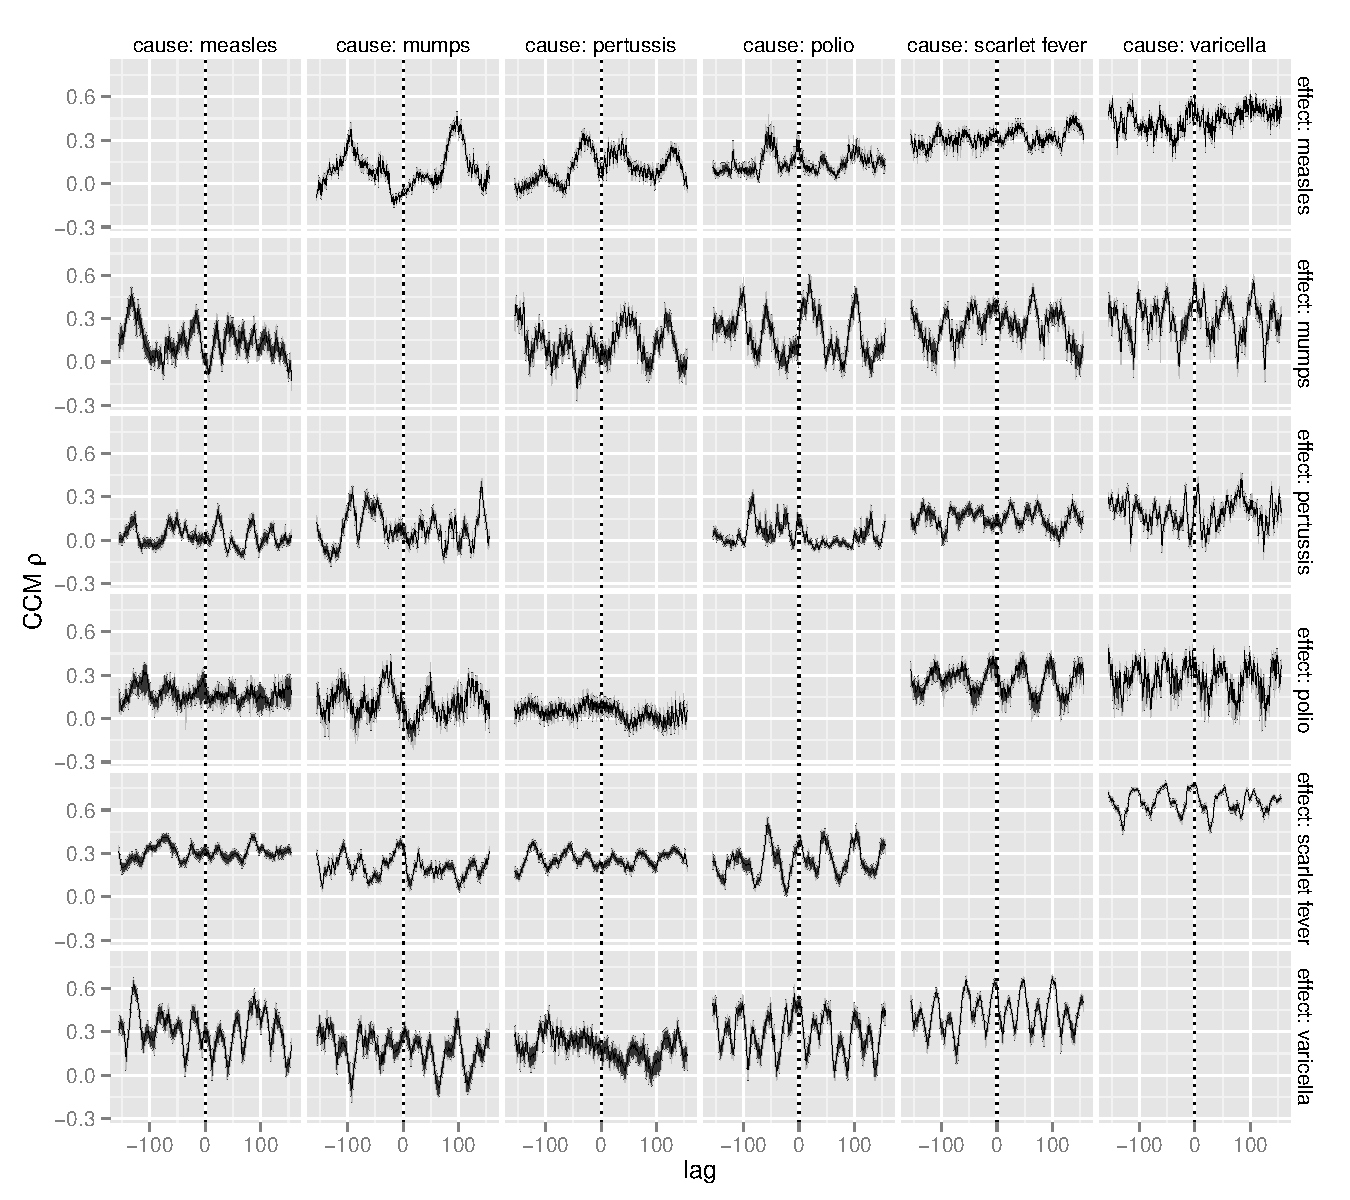
\includegraphics[width=5in]{dataflow/out/fig_cities_corrbylag/chi_self_uniform_plot.pdf}
  \end{center}
  \caption{\textbf{Cross-map lags for Chicago with default (univariate) embedding}.  \label{fig:chi_uni_tmp}}
\end{figure}

\begin{figure}
\begin{center}
  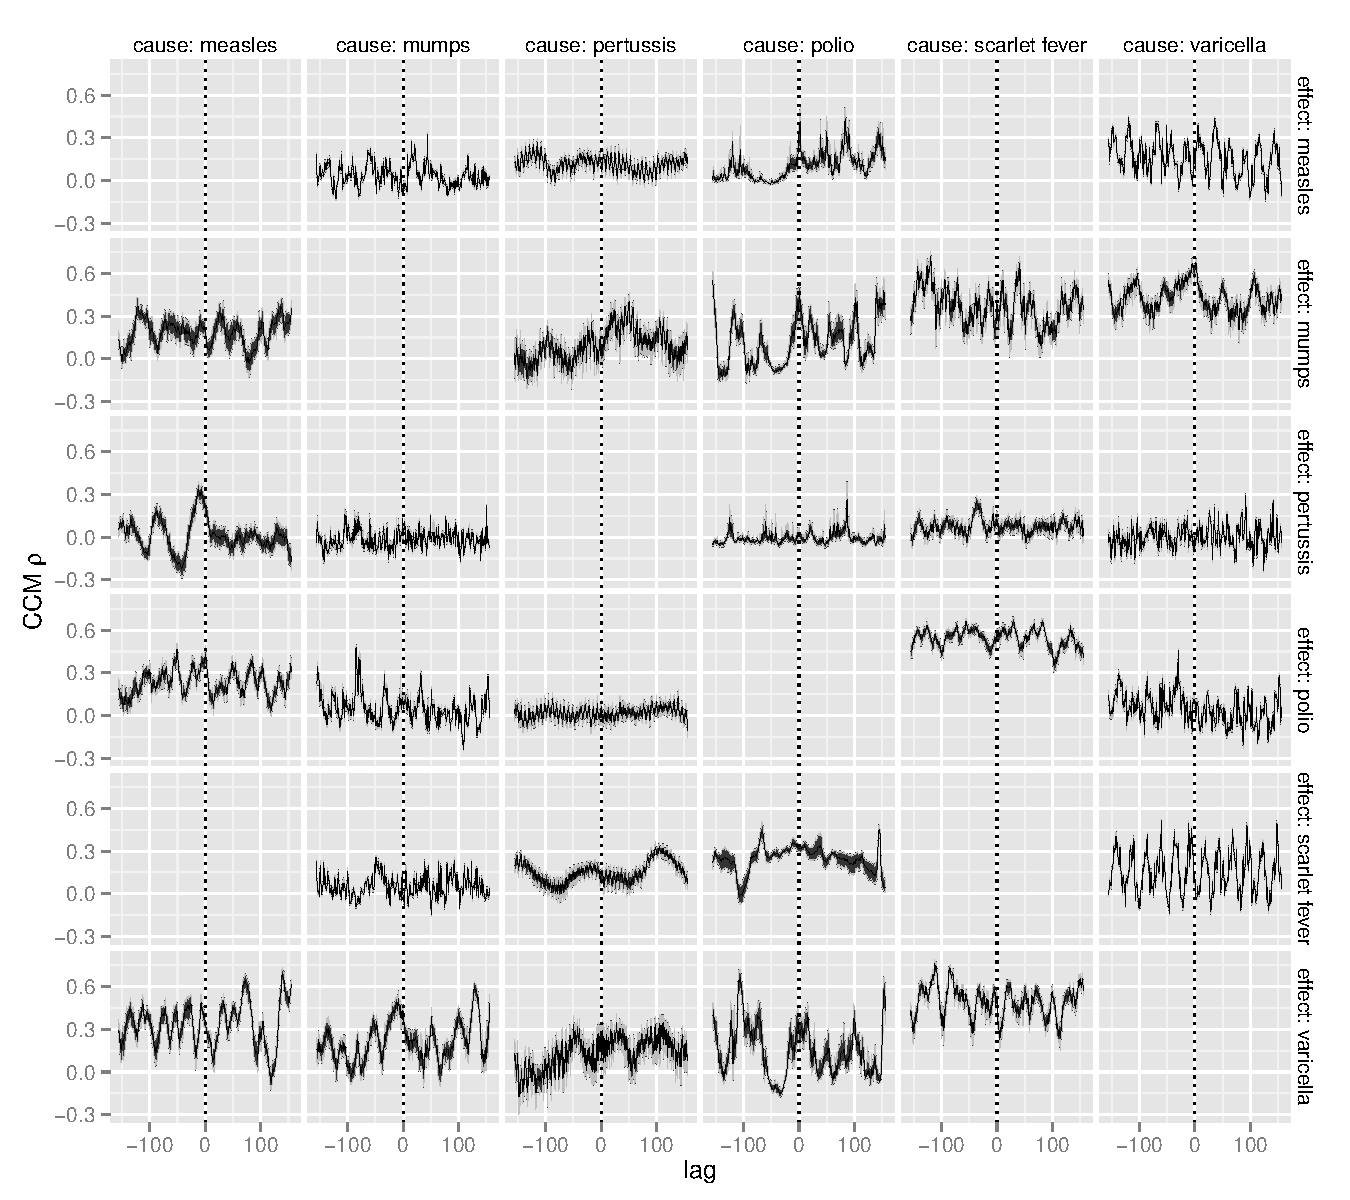
\includegraphics[width=5in]{dataflow/out/fig_cities_corrbylag/nyc_cross_projection_plot.pdf}
  \end{center}
  \caption{\textbf{Cross-map lags for New York with embedding based on random projection}.  \label{fig:nyc_rand_tmp}}
\end{figure}

\begin{figure}
\begin{center}
  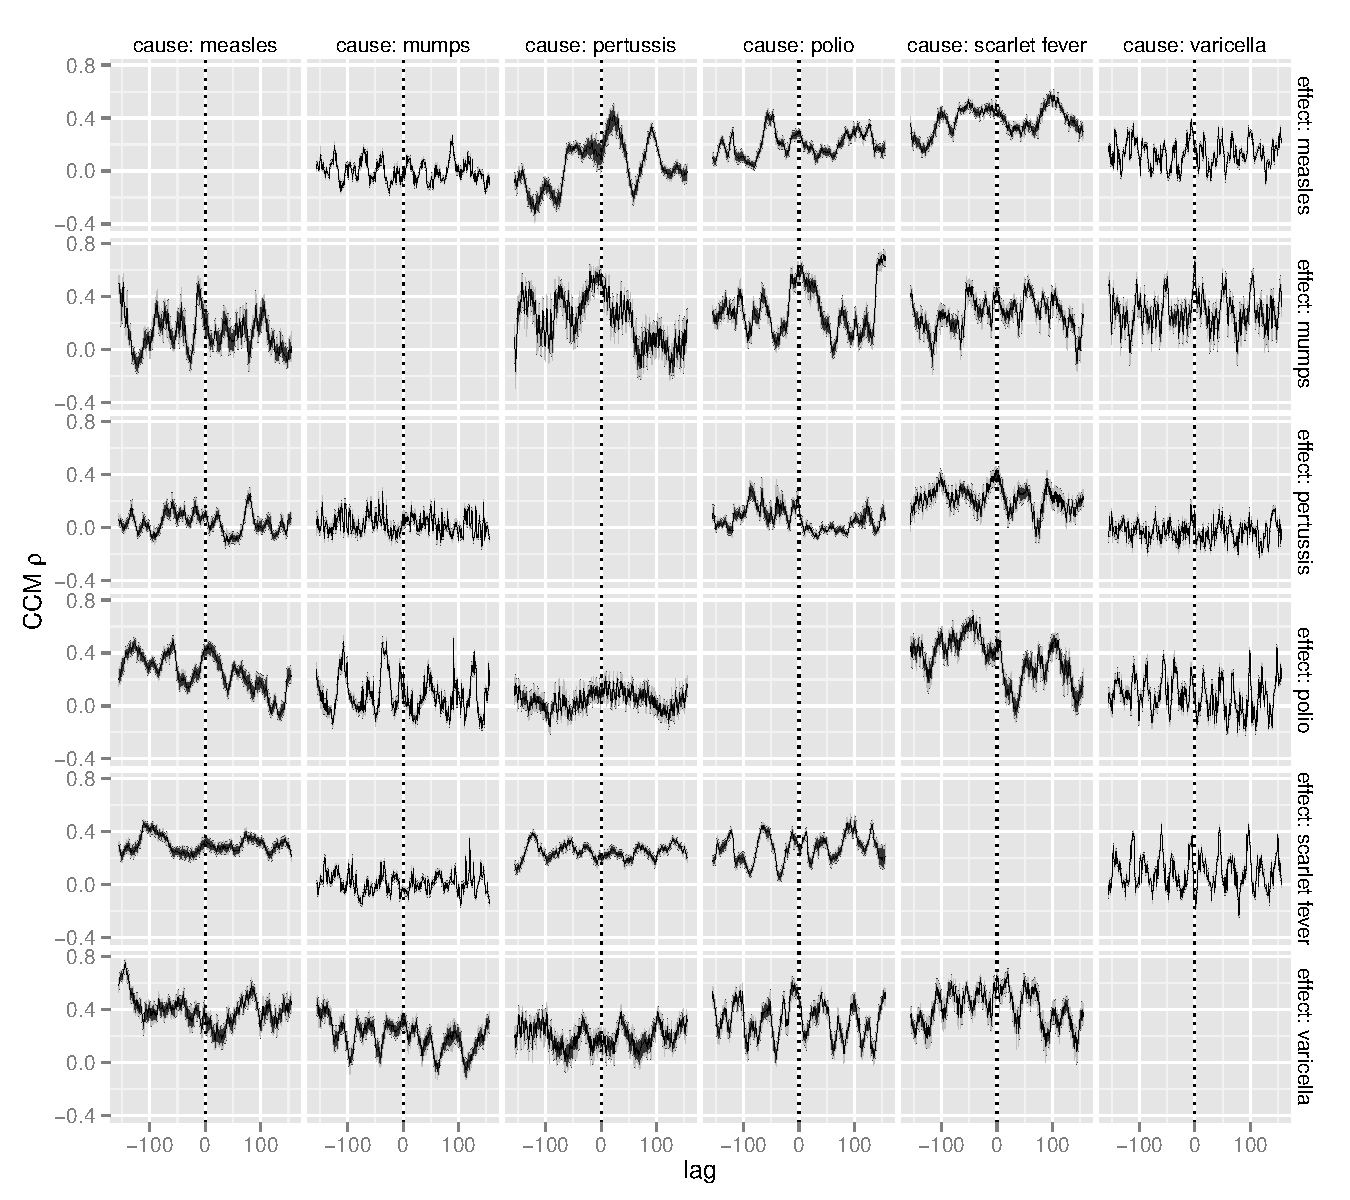
\includegraphics[width=5in]{dataflow/out/fig_cities_corrbylag/chi_cross_projection_plot.pdf}
  \end{center}
  \caption{\textbf{Cross-map lags for Chicago with embedding based on random projection}.  \label{fig:chi_rand_tmp}}
\end{figure}



\end{document}
